\documentclass[10pt]{article}
\usepackage[UTF8]{ctex}
% Replace `letterpaper' with`a4paper' for UK/EU standard size
\usepackage[a4paper,top=2cm,bottom=2cm,left=3cm,right=3cm,marginparwidth=1.75cm]{geometry}

% Useful packages
\usepackage{amsmath}
\usepackage{mathrsfs,amsmath}
\usepackage{graphicx}
\usepackage[colorlinks=true, allcolors=blue]{hyperref}
\usepackage{graphicx} %插入图片的宏包
\usepackage{float} %设置图片浮动位置的宏包
\usepackage{subfigure} %插入多图时用子图显示的宏包
\usepackage{parskip}
\usepackage{indentfirst} 
\setlength{\parindent}{2em}
\usepackage{hyperref}  
\usepackage{tikz}
\allowdisplaybreaks
\usepackage{multirow}
\usepackage{amsmath}
\usepackage{amsfonts,amssymb} 
\usepackage{xcolor} % 用于显示颜色
\usepackage{listings} % 用于插入代码
\lstset{
	basicstyle          =   \sffamily,          % 基本代码风格
	keywordstyle        =   \bfseries,          % 关键字风格
	commentstyle        =   \rmfamily\itshape,  % 注释的风格,斜体
	stringstyle         =   \ttfamily,  % 字符串风格
	flexiblecolumns,                % 别问为什么,加上这个
	numbers             =   left,   % 行号的位置在左边
	showspaces          =   false,  % 是否显示空格,显示了有点乱,所以不现实了
	numberstyle         =   \zihao{-5}\ttfamily,    % 行号的样式,小五号,tt等宽字体
	showstringspaces    =   false,
	captionpos          =   t,      % 这段代码的名字所呈现的位置,t指的是top上面
	frame               =   lrtb,   % 显示边框
}

\lstdefinestyle{Python}{
	language        =   Python, % 语言选Python
	basicstyle      =   \zihao{-5}\ttfamily,
	numberstyle     =   \zihao{-5}\ttfamily,
	keywordstyle    =   \color{blue},
	keywordstyle    =   [2] \color{teal},
	stringstyle     =   \color{magenta},
	commentstyle    =   \color{red}\ttfamily,
	breaklines      =   true,   % 自动换行,建议不要写太长的行
	columns         =   fixed,  % 如果不加这一句,字间距就不固定,很丑,必须加
	basewidth       =   0.5em,
}

\title{人工智能大作业第二阶段报告:基于DQN的强化学习}
\author{林子开21307110161 鞠扬21300180032 苏宇骢212300180030}
\begin{document}
	\maketitle

\paragraph*{摘要} 报告介绍了本小组基于DQN设计的太空采矿AI的原理与创新点。
首先梳理了从Q-Learning到DQN的数学原理,介绍了DQN的优势。接着介绍了本次DQN模型所采用的神经网络。
AI每一回合都从当前战局中提取七层主要特征,输入卷积神经网络,并选择神经网络估值最高的动作。
然后介绍了动作空间,本小组避免让AI直接操作繁琐的飞行指令细节,而为AI提供了模块化封装的动作“组合拳”,优化了动作空间。
在奖励函数的设计上,我们则根据各要素的重要性变化重构了奖励函数,并引入了人类的先验知识,对AI的行为进行额外奖励。
报告最后指出了现阶段AI的不足之处,并规划了下一阶段的改进方案。

	% \tableofcontents

\section{太空采矿游戏概述}
Kore是一项双人完全信息博弈游戏。双方在宇宙中生产战舰,扩建船厂,开采矿石,并攻击对手。
在400回合之内消灭对手的一方,或在400回合后拥有矿石数量更多的一方将会获胜。

在游戏起始时,双方都各自拥有一个船厂和500份矿石。建造一艘战舰需要10份矿石,而建造一个船厂需花费50艘战舰。

双方的智能体只能够向所拥有的船厂下达两类指令:生产战舰,或者派出一个舰队。掌握一个船厂越久,
则可以一回合中可以生产越多的战舰。每个舰队至少要包含一艘战舰,舰队能够执行的策略指令的长度,
与舰队中战舰数量正相关。

双方的舰队将在航行的过程中不断收集矿石。越小的舰队有越高的采矿效率。但是,在宇宙中也可能遇到地方战舰,
则此时会发生相撞。发生相撞时,舰队规模较大的一方(如果规模相等,则携带矿石数量较多的一方)将会胜利,
并攫取失败一方的所有矿石。

宇宙中的矿石会不断增长。但是,如果在某个位置建立船厂,则该位置的矿石会被销毁。当两艘战舰对撞,
如果双方战舰数量相等且携带矿石数量相等,则各自携带的矿石则会留在对应位置。

此外,智能体能够看到对方的所有基本信息,包括各舰队的飞行计划、携带矿石数量、舰队规模,各船厂的
每回合最大生产战舰数量,拥有的战舰等。

以上即为太空采矿游戏的基本情况。
具体的规则请参考\href{https://www.kaggle.com/competitions/sds-ai-kore/overview}{Kore游戏的官方说明}。


\section{DQN介绍}
我们使用了Deep Q-learning,也称Deep Q-network(简称DQN)作为强化学习的底层算法。从数学原理上看,DQN使用了随机梯度下降的方式,
近似求解\textbf{贝尔曼最优方程}。从模型特点上看,DQN使用了\textbf{两个神经网络}(main network 与 target network)异步更新,
并从\textbf{经验池}(replay buffer)中抽取样本进行训练,能够使学习过程较为稳定,收敛较快。
以下是我们对DQN的三个要点的介绍。

\subsection{Q-Learning原理}
首先,我们对Q-Learning进行简要介绍。
Q-Learning是一种模型无关的强化学习算法,能够同时找出最优动作估值$Q^*(s,a)$和最优策略$\pi^*$。其更新公式如下:
\begin{align}
Q_{t+1}(s_t,a_t) = Q_{t}(s_t,a_t) - \alpha_t \left[ Q_t(s_t,a_t) - \left(r_{t+1} + \gamma \mathop{\max}_{a\in \mathcal{A}(s_{t+1})} Q_t(s_{t+1},a) \right)  \right]	
\end{align}
其中$\alpha_t$是学习率,会逐渐衰减。
从数学本质上看,Q-Learning使用了随机近似的算法,求解了以下方程
\begin{align}
	Q(s,a) = \mathbb{E}\left[ r_{t+1} + \gamma \mathop{\max}_{a\in \mathcal{A}(s_{t+1})} Q_t(s_{t+1},a) \Big| s_t=s,a_t=a \right]
\end{align}
该方程就是著名的\textbf{贝尔曼最优方程}。

值得一提的是,Q-Learning既可以使用同策略(on-policy)学习,也可以进行异策略(off-policy)学习。在本次大作业中,本小组使用的是\textbf{异策略}学习,
允许AI从别的智能体的对战经验中学习策略。

\subsection{函数近似}
最简单的实现Q-Learning的方式,就是将动作价值$Q(s,a)$存储在一个表(Q-table)中,
但是这种基于表格的Q-Learning常受限于巨大的状态和动作空间的数目,而且也缺乏泛化能力。
为了解决上述问题,可以使用近似函数来逼近动作价值,即$\hat{Q}(s,a;w)\approx Q(s,a)$,其中$w$是近似函数的参数。
利用近似函数逼近真实值的方法往往具备很好的加速效果。
此外,通过对早期经验的学习,近似函数也可以在一些未出现的状态中展现出较好的泛化能力。于是,引入近似函数后的Q-learning,
实际上是在对近似函数的参数$w$进行更新。

\subsection{Deep Q-learning的特点:双神经网络与经验回放}
在各种近似函数中,如果选择神经网络,把深度神经网络与Q-Learning融合起来,就得到了DQN的方法。
对于较为简单的简单任务,甚至不一定需要深度神经网络;具有两三个隐藏层的浅层网络可能就已经足够高效。
对于一个具有较好近似效果的神经网络,我们希望它能够尽可能精确地逼近贝尔曼最优方程的解,也就是
$r + \gamma \mathop{\max}_{a\in \mathcal{A}(s')}\hat{Q}(s',a;w)-\hat{Q}(s,a;w)\approx 0$.  

为达到上述目标,我们要求神经网络最小化以下损失函数的期望:
\begin{align}
J = \mathbb{E} \left[ \mathcal{L}\left(r + \gamma \mathop{\max}_{a\in \mathcal{A}(s')}\hat{Q}(s',a;w)\,,\,\hat{Q}(s,a;w)  \right)  \right]	
\end{align}
其中损失函数$\mathcal{L}(\cdot,\,\cdot)$我们选用了Huber损失函数,该损失函数兼具MSE和MAE的优点。

在最小化目标函数$J$的过程中,DQN还使用了以下两项重要的技术:

第一项技术是使用主网络和目标网络,并进行异步更新。主网络用于给出对$\hat{Q}(s,a;w)$的估计值,并且频繁更新;
而目标网络则在短期内保持不变,用于给出$r + \gamma \mathop{\max}_{a\in \mathcal{A}(s')}\hat{Q}(s',a;w)$的估计值。
在每次迭代中,我们从经验池(replay buffer)中按照均匀分布随机抽样出一批样本$\{(s_t,a_t,r_t,s_{t+1})\}$输入主网络。
主网络给出估计值$\hat{Q}(s,a;w)$,目标网络给出目标值$r + \gamma \mathop{\max}_{a\in \mathcal{A}(s')}\hat{Q}(s',a;w)$,
然后使用随机梯度下降的方式,最小化损失函数的期望。在一定轮次之后,将主网络的权重覆盖到目标网络上。

第二项技术是经验回放(experience replay)。
当我们收集一些经验样本后,我们不按照收集的顺序来使用它们,而是将它们储存在经验池里。每次更新主网络时,
我们按照均匀分布从经验池中提取一组样本(batch)。
尽管样本是贯序收集的,相邻样本之间具有显著的相关性,但是使用抽样的方式,
则可以打破样本间的前后相关性,让神经网络从样本中学习到更普适性的知识。
此外,通过将经验保存在经验池中,每个经验都可以被多次学习,也提高了经验利用率。

DQN的示意图如图\ref{dqn}所示:
\begin{figure}[H]
	\centering
	{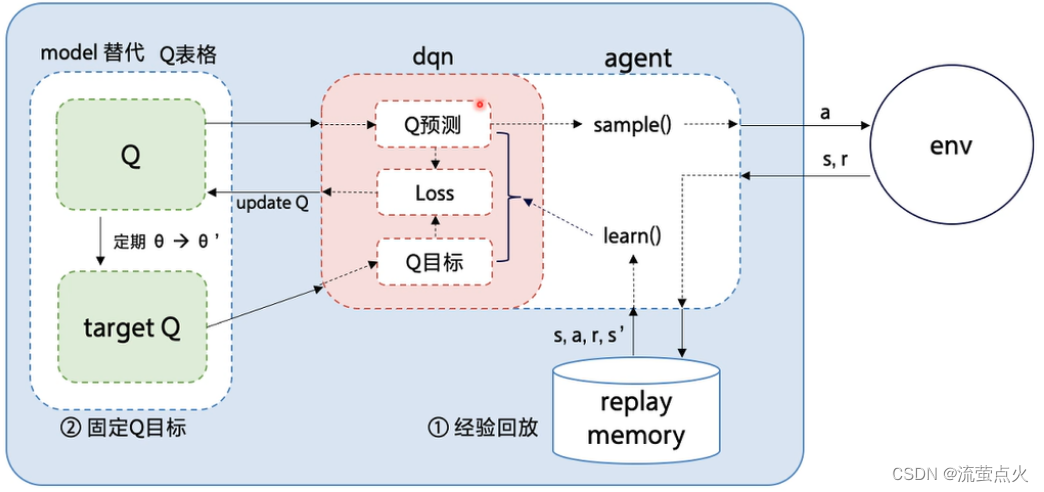
\includegraphics[width=0.5\textwidth]{image//DQN示意图.png}} 
	\caption{DQN学习流程示意图} \label{dqn}
\end{figure}

\section{神经网络与特征提取}

\subsection{神经网络结构}
为提高泛化能力,我们先人为从战场状况中提取7大特征作为神经网络的输入$s$(7个特征的介绍详后)。
神经网络共包含两个卷积层,一个展平层,两个全连接层。
输出层有五个节点,各节点的输出值代表在当前局面下选择该节点对应的动作$a_i$的价值估计值$\hat{Q}(s,a_i)$。损失函数则采用Huber损失函数。
由于本小组同学尚未修读神经网络相关课程,对神经网络领域的知识暂时不熟悉,
因此该神经网络的设计参考了\href{https://keras.io/examples/rl/deep_q_network_breakout/}{keras官方文档中的示例},特此说明。

以下是对我们人为提取的7个特征的详细介绍。

\subsection{七层特征}

我们提取以下7个战场特征,构成$21\times 21 \times 7$的张量,输入神经网络对$Q(s,a_i)$进行拟合:
\begin{enumerate}
	\item \textbf{天然矿石}:各个位置上的天然矿石数量,不包含舰队所携带的矿石;
	\item \textbf{战舰规模}:各个位置上的舰队所拥有的战舰数量,以及各个位置的船厂内已生产的战舰数量,分别用正数表示我方的战舰数量,用负数表示敌方战舰数量,
				若此处没有舰队也没有船厂,则用0表示;
	\item \textbf{舰队分布}:所有舰队当前的位置,用$+1$表示我方舰队,用$-1$表示敌方舰队,用$0$表示此处无舰队;
	\item \textbf{已采矿石}:各个位置上的舰队所携带的矿石数量,不对敌我进行区分,若该位置没有舰队,则用$0$表示;
	\item \textbf{船厂分布}:所有船厂的位置以及该船厂回合最大可造船数(该值越大则说明船厂被控制了越久,对于玩家来说重要程度越高),用正数表示我方船厂,用负数表示敌方船厂;
	\item \textbf{敌方舰队动向}:敌方所有舰队下一步移动位置,用$-1$表示,若该位置敌方舰队不会到达,则用$0$表示;
	\item \textbf{我方舰队动向}:所有舰队下一步移动位置,用$+1$表示,若该位置我方舰队不会到达,则用$0$表示。
\end{enumerate}

注:对于天然矿石、战舰规模、已采矿石这三个特征,由于其数值较大,于是我们
将各个位置的数值都除以我们估计的最大值(我们预估$5000$),将其映射到$[0,1]$区间或$[-1,1]$区间,以便于神经网络更好地对我们提取的特征进行学习。

神经网络的结构如图\ref{network}所示:
\begin{figure}[H]
	\centering
	{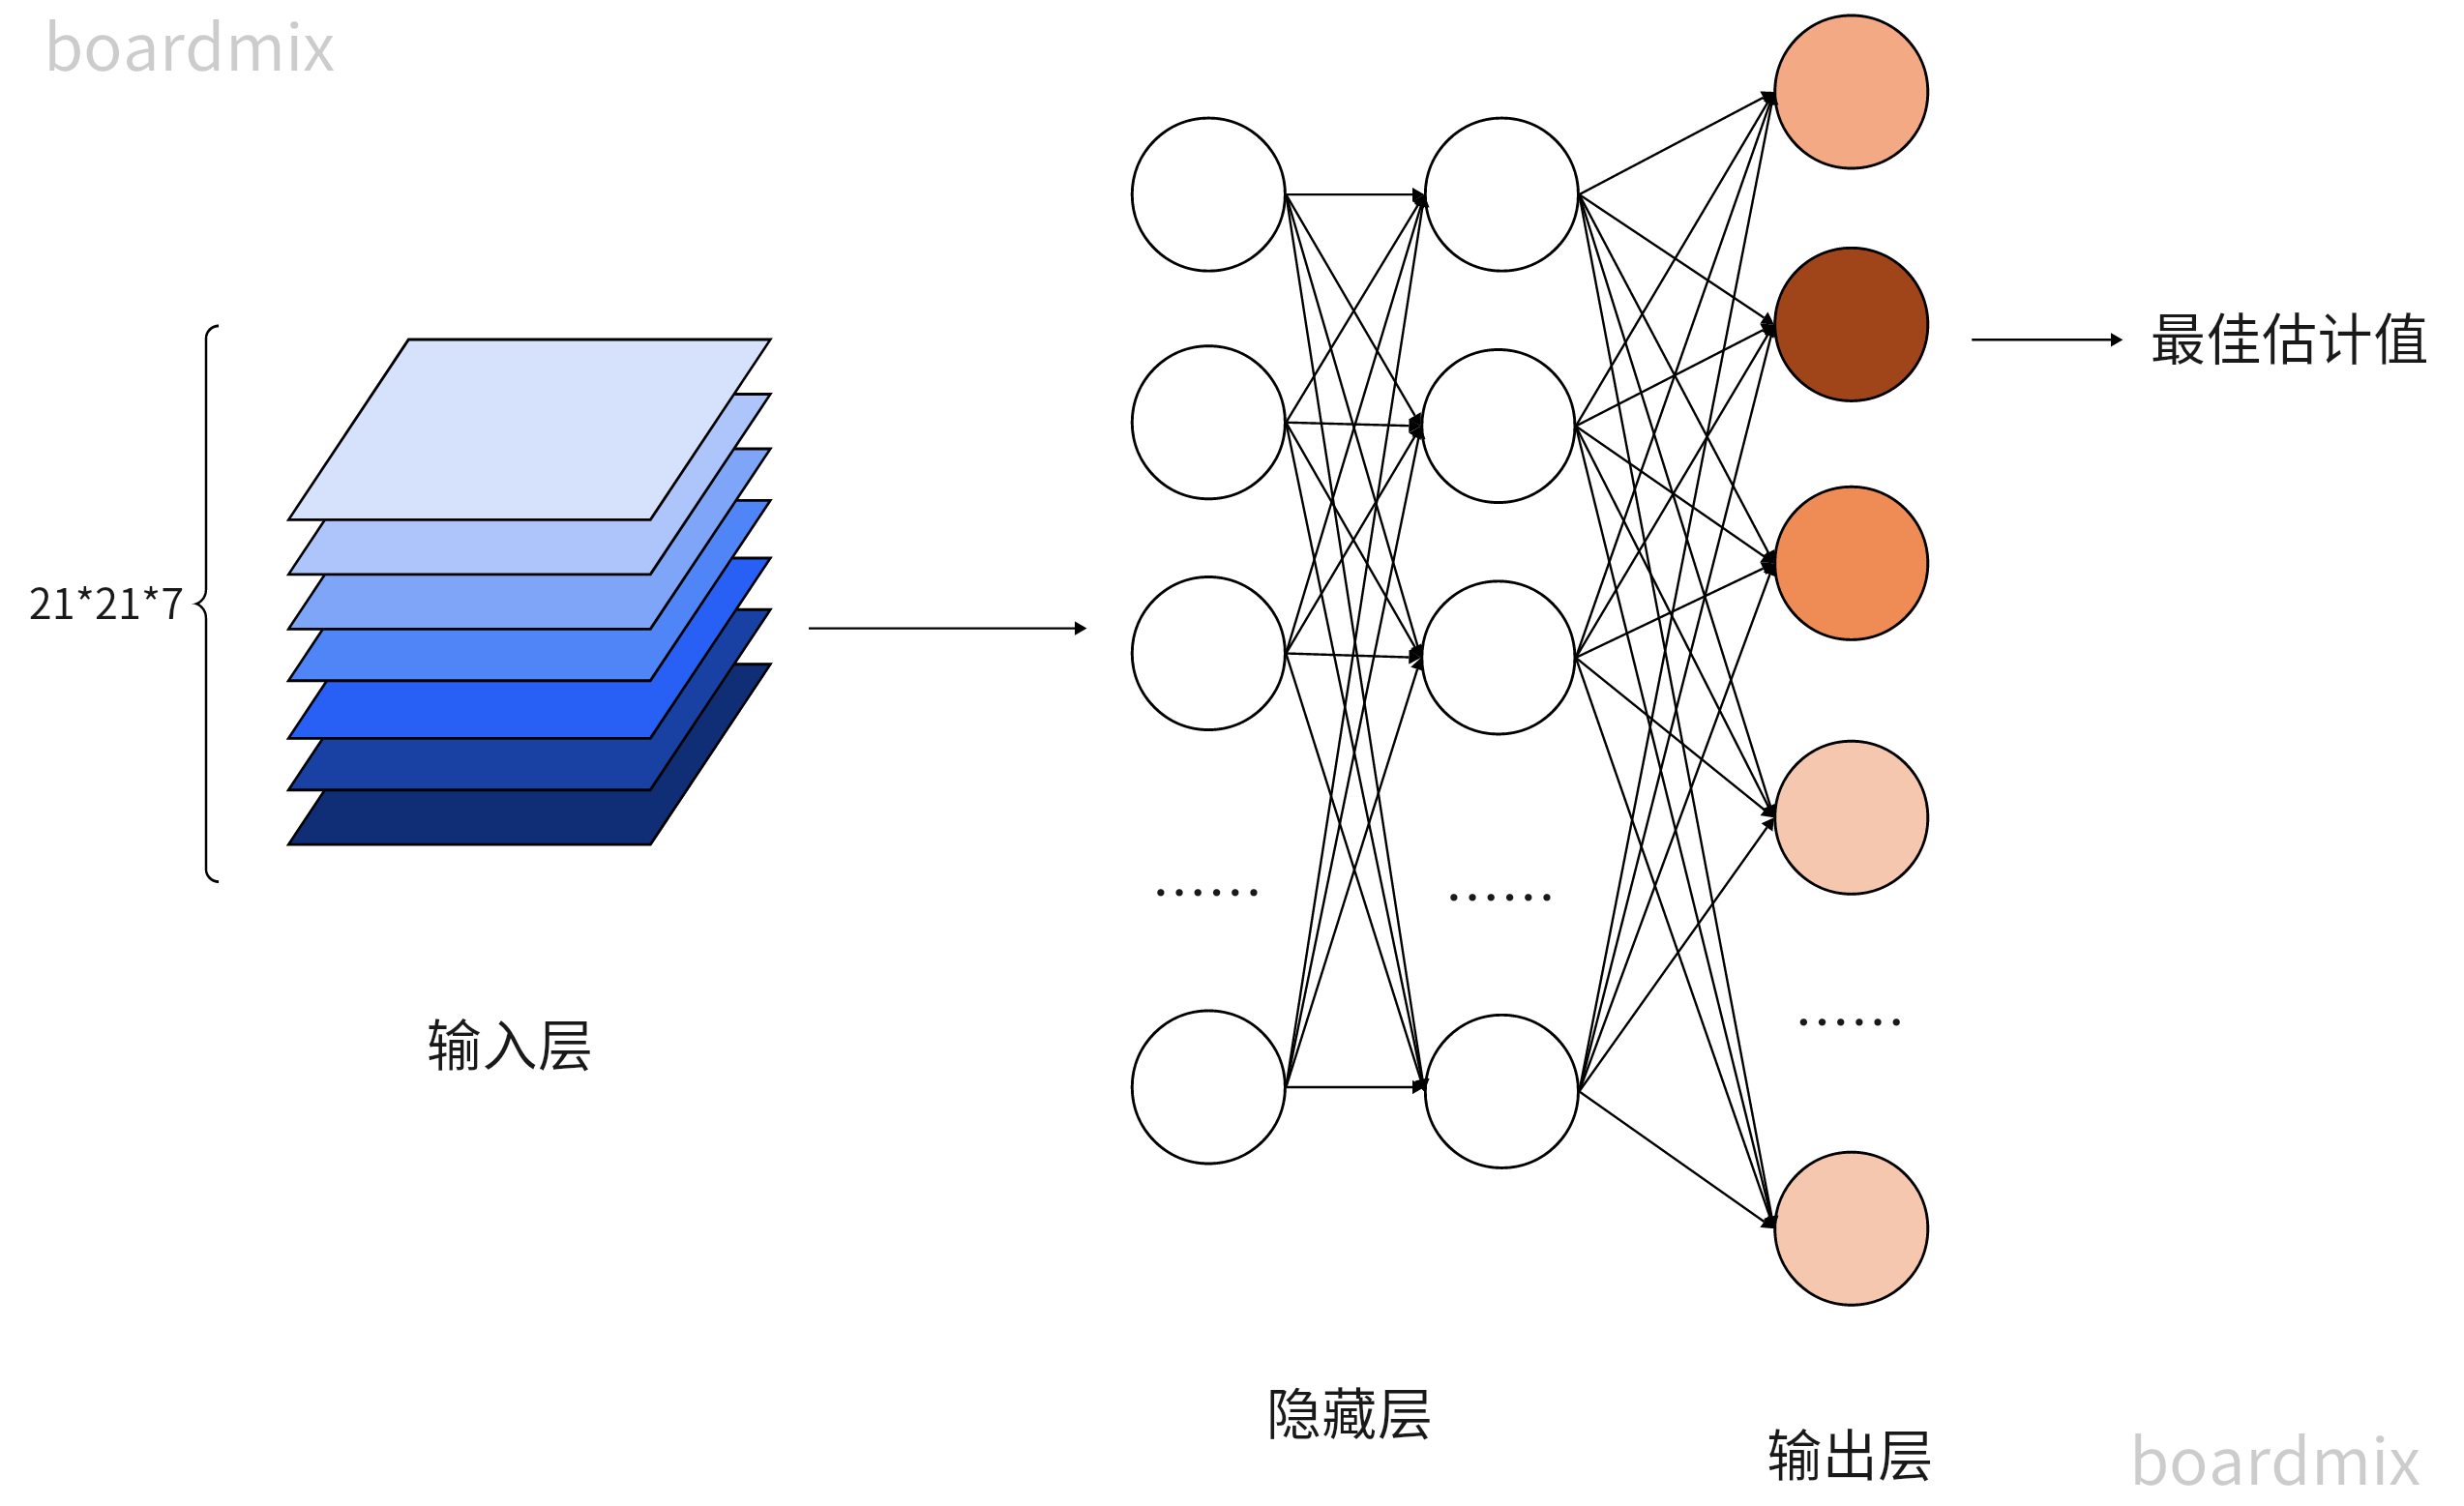
\includegraphics[width=0.5\textwidth]{image//神经网络示意图.png}} 
	\caption{神经网络示意图} \label{network} 
\end{figure}


% 游戏数值设定:
% 1.	战场中天然矿石数量的最大值为500
% 2.	每支舰队的最大规模为1000艘飞船
% 3.	每支舰队所能携带矿石的最大数量为5000

\section{智能体动作设计}

在建立强化学习模型的过程中,我们发现,直接让AI学会制定各个船厂的具体指令十分困难。比如,AI基本无法学会制定出
“N10E5C”“N5E6S5W”这类精巧复杂的舰队指令。于是我们转变了思路,为AI提供抽象层次上的动作,也即一些封装成模块的动作。
打个比方,冲拳、踢腿、空翻、虚步、劈拳、别肘等是中国传统武术中的基本动作,但是我们的AI难以直接学会这些底层的具体动作。
不过,如果将这些基本动作采用不同的顺序组合在一起,就可能成为少林拳、武当拳、八卦拳、迷踪拳、闪电五连鞭等多种拳法,
往往能体现出四两拨千斤的惊人效果!而我们提供给AI的“动作”,就是封装后的“组合拳法”。

具体而言,我们提取并总结出了5套“组合拳法”,即\textbf{优先进攻、优先挖矿、优先扩张、优先防御、中庸之道},让AI根据战场状况,
选择最适合的组合拳法。

接下来对这五套组合拳进行介绍。优先进攻、优先挖矿、优先扩张、优先防御,这四套拳法的“原料”是相同的,即
攻击、采矿、扩建、防御四个基本动作,但优先级不同。我们\textbf{以优先进攻为例}进行介绍。当AI选择优先进攻时,
会对我方\textbf{每一个船厂}依次按照下述动作顺序进行考虑:
\begin{itemize}
	\item \textbf{攻击}:首先评估该船厂是否应该攻击距离最近的敌方船厂。当同时满足以下条件:
		距离我方最近的敌方船厂规模小,距离足够近,我方船厂船只数量达到攻击舰队设定的阈值,剩余矿石足够再次造船,
		游戏时长足够,敌方船厂距离本方船厂过近已造成形成威胁,则认为满足攻击条件,应该考虑进攻。此时,派出攻击舰队攻击距离最近的敌方船厂;
		若当前该船厂船只数量不足以形成攻击舰队,则在该船厂中建造尽可能多的船只。

	\item \textbf{防御}:若该船厂经过评估,不适合进行攻击,则评估是否应该进行防御。若该船厂的附近区域出现敌方舰队,
		且敌方舰队船只数量充足,有击毁我方船厂的能力时,则认为应当进行防御,加强自身抗打击能力,在原船厂中尽可能多地建造船只。
	
	\item \textbf{扩张}:若该船厂经过评估,无需进行防御,则评估是否应当扩建船厂。
		当剩余矿石充足,且船厂生产能力满足要求时,则认为满足扩建的条件。若当前船厂内船只数量足够建立新的船厂,则根据矿石分布寻找附近最优的建厂位置,
		继而派出部分舰队执行建立船厂任务;否则在原船厂中尽可能建造最多的船只。
	
	\item \textbf{采矿}:若该船厂经过评估,不适合进行扩张,则评估该船厂是否该派出舰队进行采矿。
		当船厂内战舰的数量经过评估,已经达到了最佳挖矿舰队规模时,则进行采矿。
		AI将同时考虑时间成本和预期收益,规划出最优飞行路线,并派出舰队执行采矿任务。
	
	\item \textbf{绝处逢生}:若以上四种动作的执行条件均未满足,则很有可能说明当前船厂的境遇非常糟糕,有可能会被攻陷,
		此时将依次考虑以下备用策略:
		先尝试在该船厂中尽可能建造最多的船只;如果发现连建造船只都不合时宜,则会将船厂中所有船只派出,一路向北,暗度陈仓。
\end{itemize}
对于优先挖矿、优先扩张、优先防御这三种“组合拳”,则会按照相应的优先级顺序考虑以上的四种动作,此处不再赘述。

最后一个“组合拳”是“中庸之道”,行动模式相对平衡,会均衡地使用攻击敌人、扩建船厂、最优路线采矿、建造战舰等动作。

\section{训练过程简介}
我们让我们的AI与官方提供的balanced,miner,attacker,box-miner等智能体都进行了多轮博弈,
同时也让AI与自己进行对抗博弈。为AI提供多种对手,也有利于提高AI的泛化能力。

在训练的过程中,我们采用$\epsilon$-greedy的策略,让$\epsilon$从1逐渐下降到0.2,并维持在0.2,
以使AI保持相对较高的探索性。在$\epsilon$稳定后,在$80\%$的情况下,AI会根据神经网络的估值$\hat{Q}(s,a_i;w)$,选择动作价值最高的动作$a_i$,
在$20\%$的情况下,AI则会随机出招。我们会记录下每一回合的样本$(s_t,a_t,r_t,s_{t+1})$,存入经验池。

我们每隔4个回合就对主网络进行一次训练,从经验池中按均匀分布随机选取32个样本,用于主网络的训练。
我们每隔400个回合用主网络覆盖目标网络,并保存神经网络权重。

在本地训练完毕后,我们设置$\epsilon=0$,并把神经网络的权重与AI一起上传到kaggle官网。kaggle官网上的AI
将在每一回合把战局状态输入神经网络,并执行神经网络估值最优的动作。

% \section{实战情况统计}
% 截止2023年11月30日晚上22:30,我们在kaggle上所提交的AI中的得分最高者(submission ID:34979949)获得分数1705分,
% 与其他三个测试AI的对战情况汇总如下:
% \begin{itemize}
% 	\item 我方AI与balanced对战:
% 	\item 我方AI与attacker对战:
% 	\item 我方AI与miner对战:
% \end{itemize}

\section{本小组创新点汇总}
\subsection{重构奖励函数}
本小组没有直接使用kaggle训练环境返回的每一步的reward,而是使用了\textbf{根据战局进程而调整各要素权重}的综合评分奖励机制。
具体而言,我们小组考虑了四种要素的价值,分别是:(1)已经开采并且运回大本营的矿石,(2)已经开采但仍然由舰队携带的矿石,
(3)舰队,以及(4)船厂。

其中,(1)已经开采并运回的矿石将在400轮对战后用于评估胜负,但在一开始就积累矿石并不那么重要,
一开始更应该把矿石用于生产船只并建造船厂,因此该要素的价值将随战局的推进,逐渐从0增加到1。(2)对于已经开采但仍然由舰队携带的矿石,
其有可能被敌方抢走,也有可能与对方舰队对撞而流失在外,也有可能因为回程时船厂被攻陷而把矿石拱手送人,因此这些矿石的价值
低于已经运回大本营的矿石,故权重低于已运回大本营的矿石的权重;此外,在游戏结束时,留在舰队上的矿石不计入总的矿石数,因此,
随着战局的推进,该要素的重要性也将下降到0。(3)对于舰队,在开始的时候可以用于采矿、扩建船厂、攻陷对方船厂和劫持对方舰队,
但是,制造战舰需要消耗矿石,且在游戏结束后这些战舰的造价并不会计入总的矿石数,因此舰队的重要性也会随着战局的推进而下降到0。
(4)类似的,船厂的重要性也会随着战局的推进逐步下降到0。此外,每回合最多能生产战舰数量反映出掌握船厂的时间,也能反映该船厂的重要程度,
因此,生产战舰能力越强的船厂,将会获得越高的评分。

对于一个给定的战场状态$B_i$,我们分别对敌我双方按照上述四个要素进行加权评分,得到我方的加权评分$V_{me}$,以及敌方的加权评分$V_{opp}$,
将二者相减则得到该战场状态下的得分$V(B_i) = V_{me} - V_{opp}$。将当前战场状态得分和上一回合的战场状态得分相减,得到
\textbf{本回合的综合奖励} $R_i = V(B_i) - B(B_{i-1})$。

对上述综合奖励,我们还引入了\textbf{人类经验知识}进行微调。基于我们对kaggle官网公开比赛情况的观察,我们发现:
(1)在战局的前半程过于鲁莽地进攻容易被偷袭,而在后半程主动进攻则可以攫取对方矿石,并降低对手造船的速度,因此,当AI在
回合数step小于200时选择进攻策略,则会被扣去1分的奖励;在回合数step大于200时选择进攻策略,则会被额外给予1分的奖励。
(2)在战局中途扩建船厂比较合适,能够扩张领地,增加造船速度,但在刚开始时过于冒进地扩建船厂会导致各船厂都很脆弱,
容易被敌方一一击破,在游戏快结束时扩建船厂意义也不大,甚至还会损失战船;
因此,当回合数大于125而小于350时,如果AI选择优先扩建船厂的策略,则会被额外给予
$1 + \min\left\{\max\left\{N_{shipyard}^{(me)} - N_{shipyard}^{(opp)}\,,\, 0\right\},\,2\right\}$的奖励,
其中$N_{shipyard}^{(me)}$是我方船厂数量,$N_{shipyard}^{(opp)}$是敌方船厂数量;但如果回合数小于125或者大于350,
则AI会被扣去1分的分数。(3)尽管采矿非常重要,但是,如果AI一味地追求在矿石数量,每回合都用贪心的策略尽可能多地采矿,
则很容易出现“短视”行为,即一直采矿而忽视建造船厂与攻击对手,最后会落入矿石很多但在400回合前就已被对手消灭的境地。
此外,根据我们的动作策略设计,无论选用哪种策略,都有一定的可能转入采矿行为,选择其他的动作策略也有可能会使矿石数目增加。
因此,我们设计了如下机制:若AI选择了优先采矿的策略,则会在原分数
加上$-0.025 * \min \left\{\max \left\{ N_{kore}^{(me)} - 1000,\, 0\right\}, 4000\right\}$ 的修正值,
其中$N_{kore}^{(me)}$是我方矿石数量。
当我方矿石数低于1000时,选择优先采矿能获得额外奖励;但当我方矿石数量大于1000时,再选择优先采矿则会被扣去分数,且矿石越多,
扣去的分数也会越多,最多会被扣去100的分数。

\subsection{设计动作组合拳}
我们为AI设置了多套“组合拳”,避免让AI陷入具体的飞行指令构造细节。让AI选择封装好的动作组合,
简化了动作空间,利于AI学习。本创新点已在上文详细阐述,此处不再赘述。

\subsection{多种对手与自对弈}
我们为AI提供了多种对手进行训练,可以促进AI博弈能力的泛化。
我们也借鉴了Alpha-zero的训练方式,让AI进行自我对抗博弈,也可以有效地提高AI的作战能力。


\section{当前不足与未来改进}
我们提供的“组合拳”虽然简化了AI的学习过程,但所谓“成也萧何,败也萧何”,封装后的“组合拳”
导致AI无法精准操作每一个船厂,限制了AI的灵活性;
此外,“组合拳”的模式只有五种,相对较少,巧妇难为无米之炊,这直接限制了AI的作战能力。
我们计划,在下一阶段为AI提供更多种类、更细颗粒度的组合拳,比如多船厂围攻敌方某一个船厂,
精准阻击对方舰队并抢走对方舰队矿石,营救我方某个受攻击船厂,声东击西,围魏救赵等等。

我们提取的7个特征,可能仍然不足以反映战场情况。我们认为可以增加的特征包括:
双方舰队会发生碰撞的位置,回不了船厂的舰队位置,靠近我方船厂的敌人舰队位置等。

我们将神经网络权重和AI一起上传到到kaggle官网后发现,我们的AI与不曾用于训练的对手交战时,会表现出策略上的盲目。
我们希望能够让我们的AI在kaggle上一边与其他对手作战,一边同时进行神经网络权重上的更新,不断在实战中从
新的对手那里学习作战经验,与时俱进。

\end{document}

% \begin{figure}[H]
% 	\centering
% 	{\includegraphics[width=0.35\textwidth]{image//ignorance.png}} 
% 	\caption{} \label{} 
% \end{figure}


% \lstinputlisting[style = Python,
% caption={Python codes},
% label = {efficient},
% linerange={110-125}]{exercise3.py} 


% \begin{figure}[H]
%     \centering
%     \subfigure[patch size = 11]
%     {\label{} \includegraphics[width=0.49\textwidth]{image//local equalization with patch size = 11.jpg}}
%     \,    
%     \subfigure[patch size = 51]
%     {\label{} \includegraphics[width=0.49\textwidth]{image//local equalization with patch size = 51.jpg}}
%     \,
%     \subfigure[patch size = 151]
%     {\label{} \includegraphics[width=0.49\textwidth]{image//local equalization with patch size = 151.jpg}}
%     \,    
%     \subfigure[patch size = 201]
%     {\label{} \includegraphics[width=0.49\textwidth]{image//local equalization with patch size = 201.jpg}}
%     \caption{local equalization with different patch sizes}\label{} 
% \end{figure}
